%You can delete all the comments after you have finished your document
%this sets up the defaults for the documents, 12pt font and A4 size. The article type sets this up as such as opposed to letter or memo.

%for the finer points LaTeX see https://en.wikibooks.org/wiki/LaTeX or http://tex.stackexchange.com/

\documentclass[12pt,a4paper]{article}
\usepackage{titlesec} %these are how we import packages, one helps set up footers and title layout
\usepackage{fancyhdr}


% !TEX TS-program = pdflatex
% !TEX encoding = UTF-8 Unicode
\usepackage[utf8]{inputenc} % set input encoding (not needed with XeLaTeX)

\usepackage{graphicx} % support the \includegraphics command and options

\usepackage[parfill]{parskip} % Activate to begin paragraphs with an empty line rather than an indent

\usepackage{url}
\usepackage{pdfpages}
\usepackage{verbatim}
\usepackage{float}

%%% PACKAGES
\usepackage{booktabs} % for much better looking tables
\usepackage{array} % for better arrays (eg matrices) in maths
\usepackage{paralist} % very flexible & customisable lists (eg. enumerate/itemize, etc.)
\usepackage{verbatim} % adds environment for commenting out blocks of text & for better verbatim
\usepackage{subfig} % make it possible to include more than one captioned figure/table in a single float
\usepackage[toc,page]{appendix}
% These packages are all incorporated in the memoir class to one degree or another...
\usepackage{placeins}

%header and footer settings
\pagestyle{fancyplain}
\fancyhf{}
\renewcommand{\headrulewidth}{0.5pt}
\renewcommand{\footrulewidth}{0.5pt}
\setlength{\headheight}{15pt}
\fancyhead[L]{Michael Gauld - 40166593}
\fancyhead[R]{ SOC10101 Honours Project}
\fancyfoot[L]{}
\fancyfoot[C]{\thepage}

%set better section layout
\makeatletter
\renewcommand\subsection{\@startsection {subsection}{1}{2mm} % name, level, indent
                               {3pt plus 2pt minus 1pt} % before skip
                               {3pt plus 0pt} % after skip
                               {\normalfont\bfseries}}
\makeatother
\makeatletter
\renewcommand\section{\@startsection {section}{1}{0mm} % name, level, indent
                               {4pt plus 2pt minus 1pt} % before skip
                               {4pt plus 0pt} % after skip
                               {\bfseries}}
\makeatother

\setcounter{secnumdepth}{4}
\setcounter{tocdepth}{4}

%this starts the document
\begin{document}

%you can import other documents into your main one, these layout the Title and Declarations on its own page.
%you might need to change these to \ if your on Microsoft Windows.
\newcommand{\HRule}{\rule{\linewidth}{0.5mm}}

\begin{titlepage}
	\begin{center}

	\HRule \\[0.4cm]
    	{\Large \bfseries StripMine - Argument Analysis and Retrieval\par}
	\vspace{0.2cm}
	\HRule \\[1.5cm]

	
    	\vspace{3cm}
	\begin{minipage}{0.4\textwidth}
	\begin{center} \large
        \emph{}\\
        	Michael Gauld - 40166593
				
   	 \end{center}
    	\end{minipage}
	
	\vspace{2cm}
    	\begin{minipage}{1\textwidth}
    	\begin{center} \large
        
		Submitted in partial fulfilment of \\
		the requirements of Edinburgh Napier University \\
		for the Degree of \\
        	BEng (Hons) Computing
    	\end{center}
    	\end{minipage}

    	\vfill

    	% Bottom of the page
	\begin{minipage}{1\textwidth}
    	\begin{center} \large
		School of Computing
    	\end{center}
    	\end{minipage}
	
	\vspace{1cm}
    	{\large \today}


	\end{center}
\end{titlepage}
%{\large Submitted in partial fulfilment of the requirements of Edinburgh Napier University for the Degree of }

\section*{Authorship Declaration}
\vspace{0.5cm}
\begin{flushleft}
I, Michael Gauld, confirm that this dissertation and the work presented in it are my own achievement.\newline

Where I have consulted the published work of others this is always clearly attributed;\newline

Where I have quoted from the work of others the source is always given. With the exception of such quotations this dissertation is entirely my own work;\newline

I have acknowledged all main sources of help; \newline

If my research follows on from previous work or is part of a larger collaborative research project I have made clear exactly what was done by others and what I have contributed myself;\newline

I have read and understand the penalties associated with Academic Misconduct.\newline

I also confirm that I have obtained informed consent from all people I have involved in the work in this dissertation following the School's ethical guidelines.\newline
\end{flushleft}

\begin{flushleft} \large
\emph{Signed:} \\

\includegraphics[scale=0.3]{Report/graphics/sig.png}
\end{flushleft}

\begin{flushleft} \large
\emph{Date: 06/08/2019} \\
\end{flushleft}

\vspace{.5cm}

\begin{flushleft} \large
\emph{Matriculation no: 40166593}  \\
\end{flushleft}
\pagebreak

\section*{General Data Protection Regulation Declaration}
\vspace{0.5cm}
\begin{flushleft}
Under the General Data Protection Regulation (GDPR) (EU) 2016/679, the University cannot disclose your grade to an unauthorised person. However, other students benefit from studying dissertations that have their grades attached. \newline

\vspace{0.5cm}

Please sign your name below one of the options below to state your preference.\newline
\vspace{0.5cm}

The University may make this dissertation, with indicative grade, available to others.\newline
\vspace{3cm}


The University may make this dissertation available to others, but the grade may not be disclosed.\newline
\vspace{3cm}


The University may not make this dissertation available to others.\newline
\end{flushleft}



\pagebreak

%LaTeX let you define the abstract separately so it wont get sucked into the main document.
\begin{abstract}

\end{abstract}
\pagebreak

\tableofcontents % is generated for you
\newpage

\listoftables
%generated in same way as figures
\newpage

\listoffigures
%you may have captions such as equations, listings etc they should all appear as required
%these are done for you as long as you use \begin{figure}[placement settings] .. bla bla ... \end{figure}
\newpage

\section*{Acknowledgements}
Insert acknowledgements here
\subsection*{}
	I would like to thank my cat, dog and family.
\newpage


\section{Introduction}

\subsection{Background}
The Google Books database\footnote{\url{https://books.google.com}} contains scans of approximately 25 million books, and with non-fiction making up a portion of that figure, a large number of opinions and views on an extensive variety of topics is contained within them (Somers, 2017). In the field of linguistics, the presentation of claims and evidence forms the basis of what is referred to as an ``arguement''. Although identifying arguments can be a relatively trivial job for a human, it would be infeasible to have a project attempting to catalogue every argument ever made in written text. To have a software solution that is able to identify arguments accurately would make this goal far more feasible, and as a result, research into argumentation has become a topic of interest in AI.

The target audience for the deliverables is to assist those who are researching and developing software involving argumentation. The importance of this project is so that researchers can have a software solution to facilitate the analysis of text for arguments from a source and work directly with a format compatible with existing tools for working with arguments.\newline

\subsection{Aim and Objectives}
The first aim of this dissertation is to provide a background of argumentation in natural language. To achieve this aim, this dissertation will explain key concepts through a literature and technical review. As the subject of argumentation is an extensive area of research in linguistics, the topic will only be covered in as much detail as is required as to provide adequate content for argumentation in this project.

The second aim of this project is to develop an application to facilitate argument mining from a source of text, parse the results into a standard format (SADFace) used by Edinburgh Napier University, and present the results for use by argumentation researchers in other SADFace compliant applications. In order to achieve this aim, the following objectives must be met:
\begin{itemize}
    \item Project management techniques will need to be reviewed and an appropriate technique will be selected to form a structure for this project.
    \item A modular Python application will be developed that obtains text from a source such as a web API, facilitates argument mining software which analyses the text to identify the components of arguments, converts the produced data into the SADFace format, and inserts the standardised documents into a database for later use.
    \item A Python Flask web application which implements full-text indexing to provide a GUI to browse the database of SADFace formatted documents for use by researchers.
\end{itemize}

\subsection{Scope of the project}

The scope of this project is to develop a modular application which can facilitate argument mining software by obtaining text from a source, parsing it into a standard format, and inserting the documents into a database to be browsed through a web based GUI. Due to the complexity of developing argument mining software it is not feasible to develop argument mining software within the timescale of this project. Additionally research in argument mining software is ongoing and improvements are being made to existing solutions as well as new solutions being developed. By designing this application in a modular implementation to facilitate argument mining software, this project works to future-proof itself as new and improved argument mining software solutions will be compatible with this project if a suitable module is developed for it.

\subsection{Structure of the dissertation}

The first half of the dissertation establishes context for the project. Concepts and technologies are explored with reference to literature which provide the groundwork for the areas covered in this project. The second half of the dissertation explores the stages of the software development life-cycle.

Chapter 2 explorers literature relating to argumentation and helps us define what an argument is. Chapter 2 goes on to explores technology used in argument mining software as well as software used in the implementation of this project. Chapter 3 showcases project management decisions and actions made at the start of the project, such as deciding on the development methodology and requirements analysis. Chapter 4 covers the design and software implementation of the project. Chapter 5 provides an evaluation on the decisions made in relation to project management as well as the work done as part of the implementation. Chapter 6 provides a conclusion to this dissertation, evaluating if and how the aims set in this chapter have been met, as well as covering possible future work and the authors thoughts on this project.

\newpage


\section{Background}

\subsection{Introduction}

This sections aims to provide the relevant background context for this project. This section will first look at Argumentation in natural language and decide on a definition of what will be considered an argument for this project. This section will then go on to look at the various technologies associated with this project, such as background on argument mining software, as well as software used in the development of this project.

\subsection{Arguments and Argumentation Theory}

\subsubsection{Defining an argument}
When working with arguments, it is important to decide upon a strict definition so that we can differentiate what \emph{will} be considered an argument by our definition and what \emph{will not} be considered an argument. Within the context of natural language, an argument is used to portray evidence to either criticise or support a claim (Walton, 2006). 

The structure of arguments is described by Van Eemeren et al. as a ``constellation of expressed thought contents, called \emph{propositions}'' (Van Eemeren et al. 2014. p2). Van Eemeren et al. goes on to suggest that propositions are made up of two connected components. The first component they outline is the ``subject'', which is \emph{what} you are talking about (such as a person, place or item). The second component they outline as the ``predicate'', which is what you are describing the subject \emph{as}. Gilbert presents an example of how this structure can be used in regular speech.

``Eating vegetables is good for you, and since broccoli is a vegetable, it's good for you.''(Gilbert, 2017, p3).

This example could either be used in support of someone highlighting the qualities of broccoli or to criticise someone providing a negative opinion of broccoli. There are two propositions that can be identified in the example. The first proposition states \emph{``Eating vegetables is good for you''}. Here the subject is \emph{`vegetables'} and the predicate is that \emph{`eating (them) is good for you'}. The second proposition states \emph{``broccoli is a vegetable''}. Here the subject is \emph{`broccoli'} and the predicate is that \emph{`(it) is a vegetable'}.  From here, we can see that the subject of the first proposition is referenced in the predicate of the second proposition, linking the propositions together to form what we have described as an argument.

\subsection{Natural Language Processing}
Natural language processing can be defined as creating structured data from unstructured natural text (Kreimeyer et al, 2017). Creating this structured data manually can be at best time consuming, and at worst inconsistent due to the ambiguity that comes as a result of natural language. Martinez outlines that this challenge regarding ambiguity is only amplified when attempting to design a set of rules to interpret the meaning words that can have multiple meanings depending on the surrounding context, known as \emph{'word sense disambiguation'}. For example, if we saw the word \emph{``fly''} on its own, we can't say for certain whether it is referring to the noun (`\emph{fly}' as in \emph{insect}) or the verb (`\emph{fly}' as in \emph{`to fly'}) (Martinez, 2010, p354).\newline

Collobert et al suggests four standard tasks that can be used to benchmark a NLP approach (Collobert et al, 2011). These four tasks are described below. \newline

\subsubsection{Part-Of-Speech Tagging}
Linckels and Meinel outline techniques we can use to determine the structure of sentences (Linckels et al, 2011). The first technique is \emph{'Part-Of-Speech Tagging'}, also known as \emph{tokenization}, which is the process of identifying each word in the sentence. Many standards exist for set categories that words are tagged with. Examples include singular noun (notated as `NN'), plural noun (`NNS'), adjective (`JJ') and past tense verb (`VBD')\footnote{Examples used are from the \emph{Brown} tag set.}. During the tagging process many problems can arise, one of which being words with multiple meanings such are our \emph{`fly'} example. In situations such as these, assumptions are made based on probability and on existing corpora.\newline

\subsubsection{Chunking}
Another technique we can use is creating \emph{'phrases'} or \emph{'chunks'} based on the tags we can established during the tokenization process. In our definition, sentences will be made up of at least one phrase. Similarly to tokenization, we can identify phrases based on established definitions on what phrases can be. Phrases are usually based on tags and are the focus of the phrase, such as a noun phrase, a verb phrase or an adjective phrase. Linckels and Meinel use the following example to illustrate how the sentence \emph{``Every network requires a protocol like TCP/IP.''} would be broken down into phrases as a list as such:\newline

\begin{center}
\parbox{0cm}{\begin{tabbing}
(S \= (NP \= (DT Every)\\
\> \> (NN Network))\\
\> (VP (VVZ requires)\\
\> \> (NP \= (DT a)\\
\> \> \> (NN protocol))\\
\> \> (PP (IN like)\\
\> \> \> (NN TCP/IP))))\\
\end{tabbing}}
\end{center}

Due to the ambiguity of natural language, the process of creating these phrases may not also result in a single sentence structure as seen above as different parts of the sentence can be interpreted in multiple ways. When this situation arises, decide the \emph{best} answer based on probability established by either a human or existing data. \newline

\subsubsection{Named Entity Recognition}
Proper nouns, when referred to in the context of NLP, are known as \emph{Named entities}. Named entities are words or phrases in text that represent the name of a person, place, or organisation (Tjong Kim Sang et al, 2003). Where as it was previously claimed that large gazetteers, catalogues of names and places were required for the most accurate named entity recognition, a comprehensive list of \emph{every} name would not be feasible to create due to the quantity of information and how fast it changes (Mikheev et al, 1999). \newline

As a system is tagging named entities during the NER process, it is important that entities that represent the same real world entity are identically tagged, however, as indicated by Ratinov et al, this can raise problems (Ratinov et al, 2009). The first of these is instances where named entities need to be correctly chunked, for example, where a text may contain two instances of the word ``Australia'', upon closer examination of the text they are actually two different entities, ``Australia'' and ``The bank of Australia'', and as such should be separately tagged as a location and as a organisation respectively. Secondly, we encounter the opposite problem where we require different written words to correspond to the same entity. This occurs frequently in text as it is typical for authors to refer to an entity with its full name in it's first instance, but in future using a shortened representation of the name, for example using \emph{``President Barack Obama''} at first, but then using \emph{``Obama''} throughout the remainder of the text (Chieu et al, 2002). \newline

Correctly classifying named entities which are not catalogued, such as titles of media, can prove challenging. One approach we can take is by looking at surrounding words to see if any of them imply what the named entity is, for example, if the named entity was proceeded by the word \emph{watching} or \emph{watched}, we can guess that the named entity is most likely a piece of visual media such as a movie or TV programme (Downey et al, 2010).

\subsubsection{Semantic Role Labelling}

Semantic Role Labelling, which is a form of Shallow Semantic Parsing, attempts to recognise roles for predicates within a sentence (Che et al, 2008). Roles are assigned to the arguments of a verb using a variety of tags such as agents, patients, location and direction as established in Palmer et al (2005).

\subsection{Argument Mining}

Argument mining is described by Niculae et al as the process of automatically identifying arguments within documents (Niculae et al, 2017).

\subsubsection{MARGOT}

MARGOT (Mining ARGuments frOm Text) is an argument mining system which uses machine learning and natural language processing trained using a corpus of annotated argument-focused texts covering a variety of topics (Lippi et al, 2016). The argument mining process used by MARGOT is broken into two steps:

\begin{itemize}
    \item Argumentative sentence detection
    \begin{itemize}
        \item This stage uses a classifier to identify text containing claims, and another classifier to identify text containing evidence. The text must be checked by both classifiers as phrases can be classified as both containing claims and containing evidence.
    \end{itemize}
    \item Argument component boundaries detection
    \begin{itemize}
        \item This stage uses a trained combined Support Vector Machine and Hidden Markov Model to apply claim and non-claim tokens to a sentence. Using the Stanford CoreNLP suite is used for identifying the named entity as well as other NLP related tags. 
    \end{itemize}
\end{itemize}

\paragraph{Hidden Markov Model}\mbox{}\\

A Hidden Markov Model (HMM) is a tool which has seen application in part-of-speech tagging (Kupiec, 1992). Markov models are used for representing a finite number of states with varying probability. Within the context of part-of-speech tagging, the Markov model is used for determining the category of a word. Unlike a traditional Markov model which would be trained using a corups consisting for tagged words, a \emph{hidden} Markov model is trained using a corpus of untagged words and relies on the application is an additional algorithm such as the Baum-Welch algorithm\footnote{\url{https://ocw.mit.edu/courses/aeronautics-and-astronautics/16-410-principles-of-autonomy-and-decision-making-fall-2010/lecture-notes/MIT16_410F10_lec21.pdf}}.

\paragraph{HMM using Support Vector Machine}\mbox{}\\

Support Vector Machine (SVM) is a learning technique used to find the solution with the least error based on a set of training data (Joachims, 1998). Results from a SVM are evaluated by comparing a proposed solution with a randomly selected example and calculating the difference between the error in the proposed solution and the error value provided in the training data.

Altun et al (2003) suggests that using a SVM with the HMM covers many of the weaknesses of the HMM such as limitations on typical training data and a limited scope of independent assumptions that result from a HMM.

\subsection{Reddit API}

Reddit is a social networking website which allows users to share interesting information from external sites and have other users vote "up" or "down" the content (Hanson, 2016). Content shared on Reddit come in two varieties, links to external websites, typically news articles or humorous images, and \emph{self posts}, consisting of text written by the user. Since there is no restriction on what subject areas can be covered by users, the website is broken down into various themed versions of Reddit known as ``Subreddits''.

Reddit provides an API for developers to access the sites content programatically by registering the application and following the API terms\footnote{\url{https://github.com/reddit-archive/reddit/wiki/API}}.

\subsection{Python}

Python is a high-level, interpreted, object-orientated programming language. Due to features of Python such as automatic memory management, it is ideal for small programs and prototypes (wiki.python.org, 2019). Python includes a large standard library by default, with over 180,000 additional packages developed by the Python community through repositories such as the Python Package Index, known as PyPI (pypi.org, 2019).

\subsection{MongoDB}

MongoDB is a NoSQL database program which allows for the storage of flexible JSON-like documents. MongoDB is simple to configure and use, and provides drivers for a variety of popular languages such as Python, Java and C++ (mongodb.com, 2019).

\subsection{Elasticsearch}

Elasticsearch is an open source search engine which is capable of searching a wide array of data types. Elasticsearch uses an \emph{`inverted index'}\footnote{\url{http://www.dcs.bbk.ac.uk/~dell/teaching/cc/book/ditp/ditp_ch4.pdf} EXPAND IN APPENDIX} data structure to perform full-text indexing to find every unique word in a document and all documents a word occurs in (elastic.co, 2019). 

\subsection{Web Frameworks}

\subsubsection{Flask}

Flask is a web framework that allows the server to be written in Python. Flask acts as a wrapper for Werkzeug\footnote{\url{https://palletsprojects.com/p/werkzeug/}}, a web application utility library, and Jinja\footnote{\url{https://palletsprojects.com/p/jinja/}}, a template engine.

\subsubsection{Jinja2}

Jinja2 is a template engine for Python which allows for the programmatic generation of documents, such as HTML documents for when data needs to be appended server-side.

\subsection{Other Libraries}

\subsubsection{Bootstrap}

Bootstrap is an open-source front-end framework which provides many tools which assists both prototyping and full release of applications on the web (Getbootstrap.com, 2019). By using Bootstrap in this project, we are able to minimise the time spent on web design and use that time to improve the functionality of the application.

\subsubsection{SADFace}

SADFace (Simple Argument Description Format) is a JSON-based document format used to model the various aspects and meta-data related to arguments. The aim of SADFace is the provide a format suitable for use with argument related tools for the web. The contained argument is stored as a directed graph, with the nodes representing either premises or the conclusion and the edges containing both a source and target to signify direction (Wells, 2018).

\subsubsection{PRAW}

PRAW (Python Reddit API Wrapper) is a Python package which enables simple access to Reddit's API and is compliant with Reddit's API rules.


\newpage
\section{Project Analysis}

\subsection{Requirements Analysis}

Requirements analysis is the fundamental first stage of any software development project. During this stage, time is spent evaluating the individual requirements of the various stakeholders of the project. By identifying the requirements at the start of the project, clear boundaries are set about exactly what the scope of the final product will be, so any missing stakeholder requirements can be identified during this stage (Nahar et al, 2013).

\subsubsection{Stakeholders}

Within the context of a project, a "stakeholder" is anyone with an interest or influence on the project, either a person involved during the development stage or an end user (or person affected by the work performed by the end user). The stakeholders that have been identified for this project are as follows:
\begin{itemize}
    \item The author of this document
    \begin{itemize}
        \item Being both the developer of the project and the author of this document, this stakeholder has a strong influence on the scope of this project.
    \end{itemize}
    \item Dr. Simon Wells
    \begin{itemize}
        \item Dr. Wells is closely involved with the Edinburgh Napier School of Computing's argumentation research\footnote{http://arg.napier.ac.uk/} and has acted as the supervisor for this project.
    \end{itemize}
    \item Any researcher studying argumentation
    \begin{itemize}
        \item This document and associated project may provide a basis for further research into the topics covered in this document. This is an example of where not every stakeholder cannot be questioned about their requirements as an exhausted list of every researcher with an interest in argumentation cannot exist, instead we must base their requirements off a small number of stakeholders which apply to this category.
    \end{itemize}
\end{itemize}

\subsubsection{MoSCoW}

MoSCoW is a requirements prioritisation technique which sorts all of the stakeholder's requirements into one of four categories (Miranda, 2011):

\begin{itemize}
    \item Must have.
    \begin{itemize}
        \item Requirements designated as ``must have'' are essential to the core functionality of the project. The minimum state a project must have reached to be considered `complete' would be to have all of these requirements met.
    \end{itemize}
    \item Should have.
    \begin{itemize}
        \item Although not essential to the core functionality of the project, it would be in the stakeholders best interest for these requirements to be met. These may be features to help improve the ease of use with the product and may help improve the end user's efficiency. If there is additional time/resources available once all of the ``must have'' requirements are met, these are the first requirements to be worked on afterwards.
    \end{itemize}
    \item Could have.
    \begin{itemize}
        \item Requirements designated as ``could have'' are often requirements related to improve the `Quality of life' of the end user. Requirements can end up in this category due to requiring a large amount of resources to create relative to the impact it would have on the functionality of the final product, such as aesthetics.
    \end{itemize}
    \item Won't have.
    \begin{itemize}
        \item These requirements are decided at the start of the project as being outside the scope of the project. Requirements can be identified as such for many reasons such as a lack of time or a lack of required resources to realistically met the requirements within the context of the project.
    \end{itemize}
\end{itemize}

By having a distinct list of the requirements sorted into the four categories, stakeholders will be able to easily identify if the prioritisation given to the requirements that are relevant of that stakeholder are accounted for.

\subsubsection{List of Requirements}

Shown below is the MoSCoW requirements analysis that has been preformed for this project.

\begin{table}[htbp]
    \centering
    \begin{tabular}{|p{1cm}|p{8cm}|p{2cm}|}
    \hline
    ID & Requirement & Priority\\
    \hline
    1 & Access the web to retrieve text through an existing API. & Must\\
    \hline
    2 & Perform argument mining using existing argument mining software on a text with results being stored in the SADFace format. & Must\\
    \hline
    3 & Store the results in a database. & Must\\
    \hline
    4 & Be developed in a modular structure so that aspects of the application can be swapped with alternative tools in future development. & Must\\
    \hline
    5 & Provide a web interface to access and search the database. & Must\\
    \hline
    6 & Be able to access and search the results using a full-text indexing engine. & Should\\
    \hline
    7 & Use the SADFace Python library to parse documents into the SADFace format. & Should\\
    \hline
    8 & Be able to access and search the results using a RESTFul API. & Should\\
    \hline
    9 & Access the web and retrieve text by identifying bodies of text in web pages. & Could\\
    \hline
    10 & Provide a new argument mining software solution & Won't\\
    \hline
    11 & Be able to directly open a document from the search in MonkeyPuzzle & Won't\\
    \hline
    \end{tabular}
    \caption{MoSCoW requirements prioritisation}
    \label{table:1}
\end{table}

\FloatBarrier

\subsection{Development Methodology}

For software development projects, there are a number of tried project management techniques which dictate the stages a project will go through during development. Two software development methodologies were selected as suitable for this project, which are ``Waterfall'' and ``Agile''.

\subsubsection{Waterfall Methodology}

The Waterfall software development methodology is a conventional method which follows a set of linear steps, finishing each task before starting the next task (Brindha et al, 2015). The stages in the Waterfall model are as follows:

\begin{figure}[H]
    \centering
    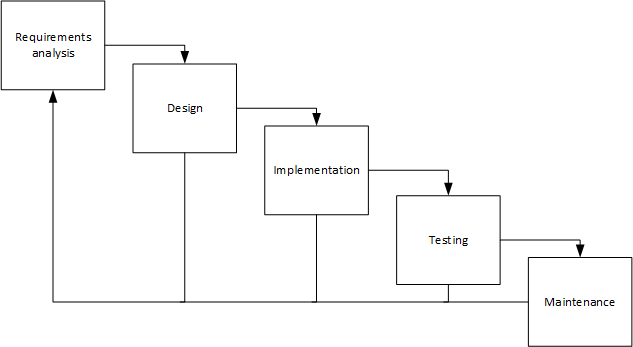
\includegraphics[scale=0.75]{Report/graphics/waterfall.png}
    \caption{Flowchart of Waterfall method}
    \label{fig:waterfall}
\end{figure}

\begin{itemize}
    \item Requirements analysis
    \begin{itemize}
        \item At the start of a project, the stakeholders are identified and the scope of the project is agreed upon.
    \end{itemize}
    \item Design
    \begin{itemize}
        \item A model is designed to show how the available technology can be used to meet the requirements.
    \end{itemize}
    \item Implementation
    \begin{itemize}
        \item The designed model is converted into a software implementation.
    \end{itemize}
    \item Testing
    \begin{itemize}
        \item Testing, such as unit testing and implementation testing are performed on the produced software.
    \end{itemize}
    \item Maintenance
    \begin{itemize}
        \item Continuous support and fixes are provided to the software depending on the arrangement between the client and the developers.
    \end{itemize}
\end{itemize}

\subsubsection{Agile Methodology}

Agile software development methodologies aim to address the common critiques of traditional development methodologies (Yu et al, 2014). One of the main critiques agile methods tackles is the traditional methods inability to adapt to changing requirements. In agile methods, the time span for the project is broken into ``sprints''.

At the start of a sprint, goals are set as to what features should be implemented during the allotted time for the sprint. At the end of the sprint the implementation of the feature should be complete and is shown to the client for feedback as to what to include in the next sprint.

\begin{figure}[H]
    \centering
    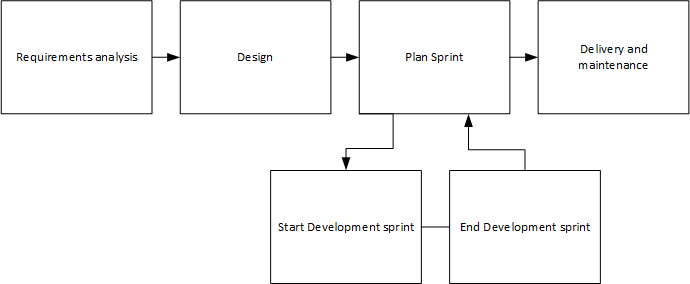
\includegraphics[scale=0.75]{Report/graphics/agile.png}
    \caption{Flowchart of Agile method}
    \label{fig:agile}
\end{figure}

\subsubsection{Methodology Comparison}

Kisielnicki et al (2017) highlights the main objectives of these two methodologies. The traditional method has a focus on processes and relies on static requirements with a linear approach to tasks. The agile method contrasts these and as it has a focus on people and can facilitate changing requirements with a flexible approach to tasks.

\begin{table}[H]
    \centering
    \begin{tabular}{|p{3cm}|p{4cm}|p{4cm}|}
    \hline
    Methodology & Fixed values & Variable values\\
    \hline
    Traditional & Features & Time and Cost\\
    \hline
    Agile & Time and Cost & Features \\
    \hline
    \end{tabular}
    \caption{Comparison of values of methodologies}
    \label{table:2}
\end{table}

\paragraph{Conclusion}\mbox{}\\

As this project has strict requirements on what \emph{must} be completed for the project to be considered a success, the traditional waterfall methodology was chosen due to its emphasis on the completion of tasks.

There are many apparent weaknesses of the traditional method, such as its inability to adapt to changing requirements and less personal approach. Being a project with a single developer and a planned short development cycle, these weakness should have a minimal impact on the project.

\newpage
\section{Design and Implementation}

\subsection{Initial Design}

Once the requirements had been established, a design was created to indicate the series of events an existing initial text source would need to be processed through to be able to be found in our argumentation database. As the software was required to be modular to accommodate new technologies in the future, stages were broken into features that could be incorporated and tested individually, and would form a full software solution when linked together.

\begin{figure}[H]
    \centering
    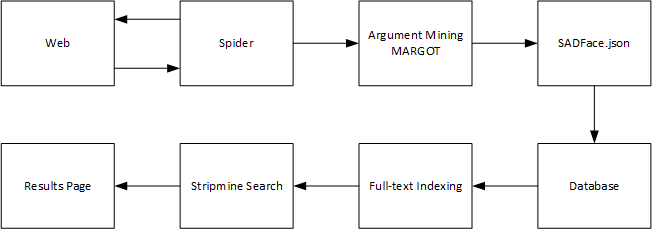
\includegraphics[scale=0.75]{Report/graphics/design.png}
    \caption{Original proposed design of Stripmine}
    \label{fig:design}
\end{figure}

\subsection{Reasoning For Choices}

\subsubsection{Python}

Python was chosen for this project for a number of reasons. Python is designed to be simple to write, making it ideal for prototypes and small projects. As the project required a short development cycle, Python is appropriate.

Python also has support for a wide range of libraries. Previous to this project, a Python library for producing SADFace formatted documents had been created\footnote{\url{https://github.com/siwells/SADFace}}. Additionally, as the software required a web component, which Flask would be suitable for, the whole application was developed in Python so code could be shared amongst the two applications if required.

\subsubsection{MongoDB}

For this project, a database would need to be used to store the produced SADFace documents. Since SADFace documents can elements that can vary, such as metadata category names, the number of nodes and number of edges, a flexible database solution was required. As the SADFace format is based on JSON, a NoSQL database solution would be most appropriate. 

MongoDB was chosen as the database software that would be used in this implementation due to it being a flexible, NoSQL database solution with existing drivers allowing it to easily interface with Python and Elasticsearch.

\subsubsection{Reddit}

Reddit (specifically the `subreddit'; ``changemyview'') was chosen to be the source of sample data for this project. Due to the nature of a social networking website such as Reddit, users are constantly producing new content which can be used as sample data resulting in there being no shortage of new data to test with.

Additionally, since Reddit posts are sorted by category, and a category exists solely for arguments meaning there would be no need to filter through the gathered data to determine if or if not the text was an argument, saving a large amount of time that can be focused on other areas of the project. As the category is arguments of any topic, a wide array of topics were covered in the testing data.

There were a small number of disadvantages of using Reddit as the source of sample data for the project. One of which is no guarantee of correct spelling and grammar.  Incorrect spelling and grammar would have an effect on the argument mining processing, causing the miner to either miss arguments which have been made, or falsely identify arguments were an argument isn't made. This disadvantage is minimised however by Reddit's ``reddiquette'' document\footnote{The ``reddiquette'' document is a list of etiquette standards expected of those who post on the site.} which encourages users to ``Use proper grammar and spelling''.

Another disadvantage is that posts users make can be edited by the user. In accordance with the ``reddiquette'' document, edited posts should include a section at the start or end of the post with ``Edit:'' followed by the changes made to the post so that it is clear to users how the post has been changed. Users also use edit feature to address questions or queries that have occurred frequently as a result of their post so that further community members do not ask the same question in a similar format to the ``Edit:'' etiquette. This ``Edit:'' (and similar sections) lead to false positives during the argument identification stage of the mining process.

\subsection{Tools Used During Implementation}

\subsubsection{PyCharm}

PyCharm is an IDE used for writing Python scripts. It allows for a sand-boxed environment for libraries and supports debugging tools. PyCharm additionally integrates with version control to track changes that have been made to documents within a project. 

\subsubsection{Version Control}

For this project, GitHub was used as version control software for this project. It allows for a backup of the project files, as well as a history of changes for each file. GitHub also features issue tracking which can be used to track existing bugs and request features.

\subsection{The Produced Software}

The implementation of this project has been split into two halves, known as ``Stripmine-Script'' and ``Stripmine-Site''. Stripmine-Script acts as a modular python script which takes in bodies of text from a source, such as the internet or books, runs the text through an argument miner, compiles the data into the SADFace format and inserts the resulting SADFace document into a database. Stripmine-Site is a Flask web-app search tool which uses full-text indexing to search and display relevant data from the database.\newline

\begin{figure}[H]
    \centering
    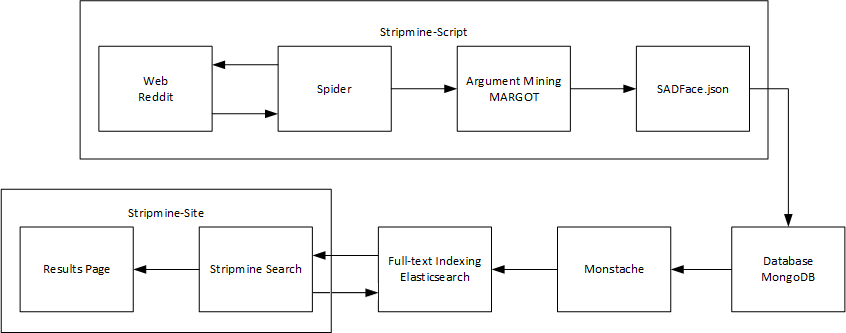
\includegraphics[scale=0.66]{Report/graphics/newdesign.png}
    \caption{Design of Stripmine in the produced software}
    \label{fig:newdesign}
\end{figure}

\subsubsection{Stripmine-Script}

This script houses four modules which can be interchanged to suit the requirements of the user. These modules are a Spider, Miner, Parser and Database. Each module exists as a python class which inherits from an abstract base class. Each of the base classes include information on how they are to be used, what to expect as inputs from the previous step in the chain, and what to output to be compatible with the next step in the chain. 

For this project, four modules have been developed and implementation to demonstrate how the software functions.

\paragraph{Spider}\mbox{}\\

The Spider class is the first module in the chain. This module obtains text from a source as well as any metadata associated with the source. The data is written to an instance of SpiderExtract, and the Spider module outputs a list of SpiderExtract items.

For this implementation the Spider accesses the Reddit API for the ``changemyview'' section\footnote{https://www.reddit.com/r/changemyview}. It obtains posts made in this section, then collects the text of these posts and relating metadata such as a link to the post, the authors username, and title of the post. The module takes this data and assigns the text and metadata to the SpiderExtract class and appends it to a list to be returned once the Spider has finished. 

\paragraph{Miner}\mbox{}\\

The Miner class accepts text gathered by the spider and runs the text through an argument miner. The argument takes this text and attempts to identify any arguments made in the text. Depending on the argument miner used, different data may be obtained. Once the argument miner has finished processing, the data is serialised into JSON format.

For this project MARGOT\footnote{\url{http://margot.disi.unibo.it/}} was used to identify and classify arguments.

\paragraph{Parser}\mbox{}\\

The Parser class works in tandem with the Miner class and an appropriate parser will need to be developed to match the miner used. The parser receives the JSON from the miner and converts the data into the SADFace format. Due to the variety of ways the miner could produce data, a parser will have to be developed to suit the data produced by the miner.

\paragraph{Database}\mbox{}\\

The Database module takes the resulting SADFace document and inserts it into a database. For this projects implmentation MongoDB was used.

\subsubsection{Monstache}

Monstache\footnote{\url{https://rwynn.github.io/monstache-site/}} is a open source tool that allows a MongoDB collection to be synchronised with an instance of Elasticsearch. This tool acts an a connector between the database from the script and the full-text indexing tool used in the site. 

\subsubsection{Stripmine-Site}

Stripmine-Site is a Flask web-app used for displaying the contents of the database containing SADFace formatted documents. The site consists of three pages, a home page, a search results page, and a document page.

\paragraph{Home Page}\mbox{}\\

The home page acts as the root of the web app. This page allows the user to enter a term to search the database for as well as filter for specific categories of arguments. The form uses a POST request to submit the data to the results page for searching.

\begin{figure}[H]
    \centering
    
\includegraphics[scale=0.5]{Report/graphics/home.png}
    \caption{Search bar from the home page of Stripmine-Site}
    \label{fig:home}
\end{figure}

\paragraph{Results Page}\mbox{}\\

This page shows the results based on the terms specified in the search that was POSTed. The results are displayed using a Bootstrap ``accordion''. The text is retrieved from the database using full-text indexing through Elasticsearch\footnote{https://www.elastic.co/}. From this page, the user can browse the arguments, view the metadata associated with the arguments presented, and further refine their search.
\newline
\begin{figure}[H]
    \centering
    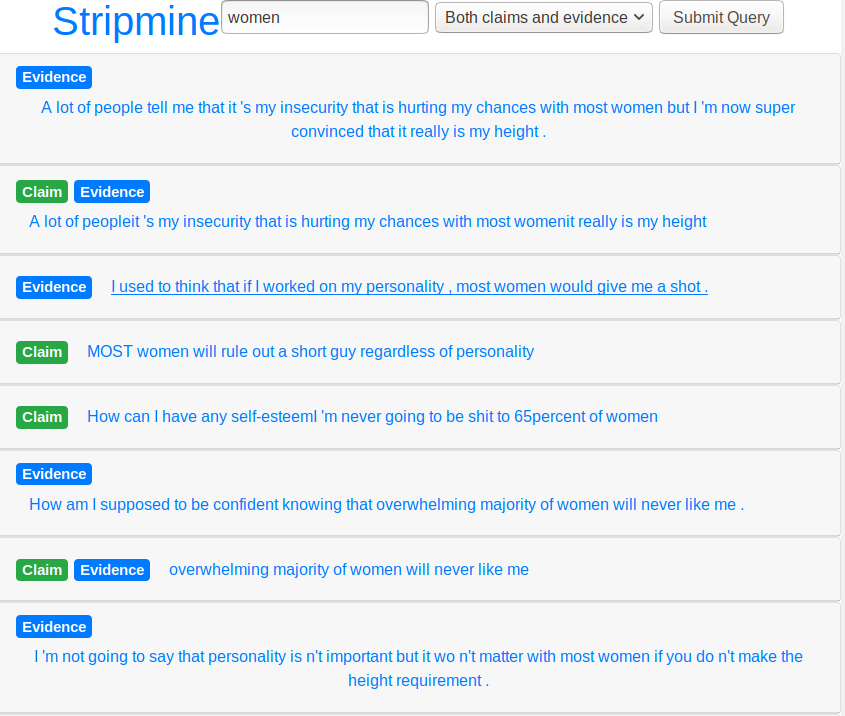
\includegraphics[scale=0.5]{Report/graphics/results-1.png}
    \caption{Results page in Stripmine-Site}
    \label{fig:results1}
\end{figure}

For each of the arguments, the user can be directed to the SADFace document which it is contained within through the document page. Since the page functions primarily through a POST request, if a GET request is received the user is redirected to the home page.

\begin{figure}[H]
    \centering
    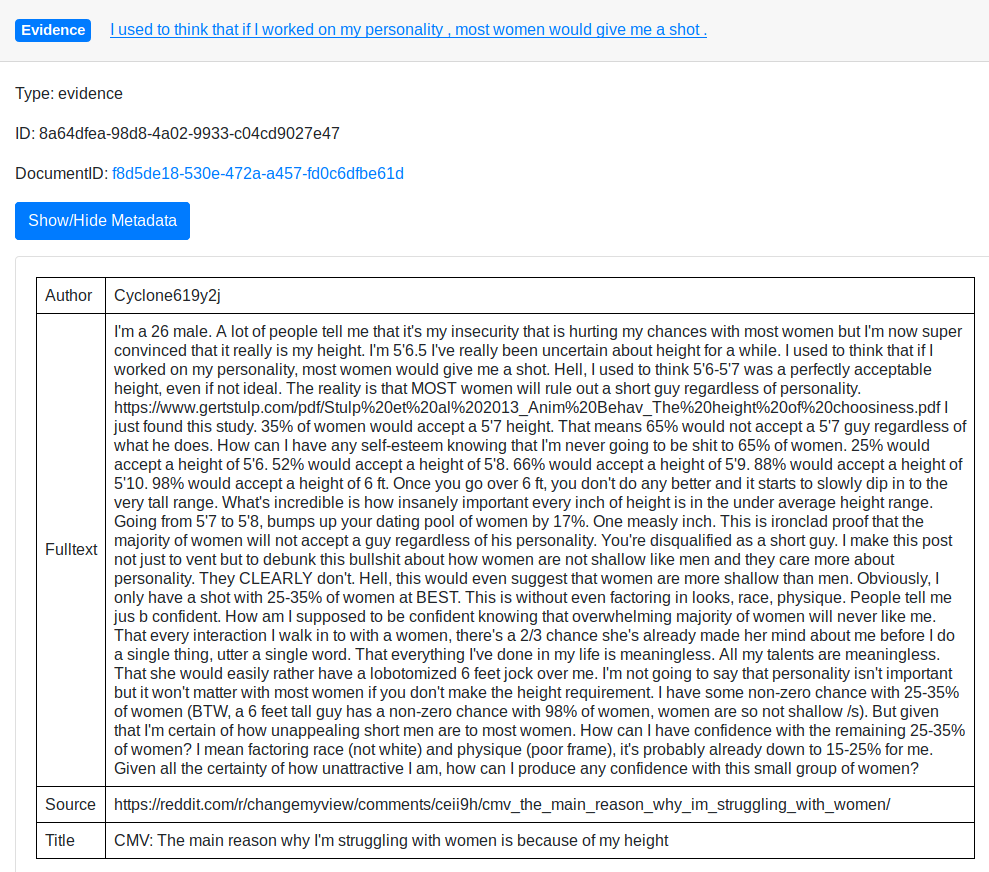
\includegraphics[scale=0.4]{Report/graphics/results-2.png}
    \caption{Selected result in results page}
    \label{fig:results2}
\end{figure}


\paragraph{Document Page}\mbox{}\\

The document page shows the full metadata and a list of all the arguments presented within a SADFace document. The associated metadata is presented at the top in a programmatically generated table displaying every metadata field and value. The arguments are presented below in the same manner as is used for the results page. A link is provided to download the SADFace document for further work in an application such as Monkeypuzzle\footnote{http://arg.napier.ac.uk/monkeypuzzle/}.

\begin{figure}[H]
    \centering
    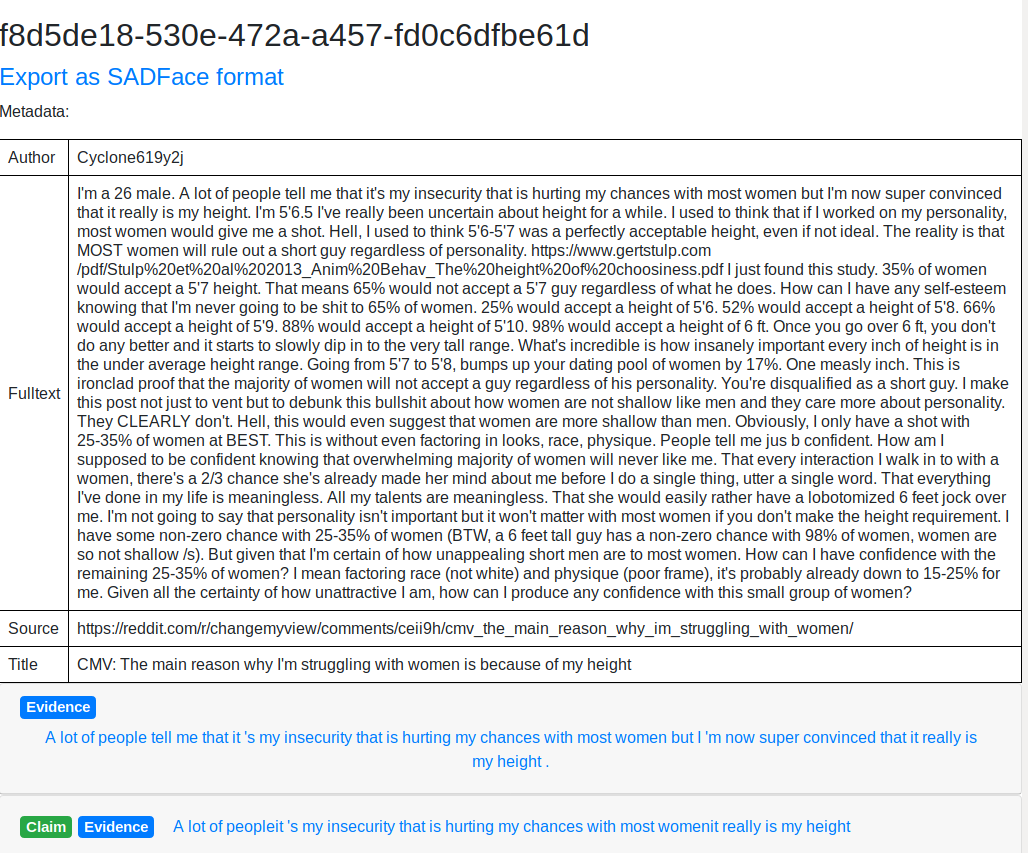
\includegraphics[scale=0.4]{Report/graphics/document.png}
    \caption{Document Page in Stripmine-Site}
    \label{fig:document}
\end{figure}

\newpage
\section{Evaluation}

\subsection{Analysis of Project Management Technique}

In Chapter 3, two project management techniques, a traditional waterfall methodology and the agile methodology, were reviewed, contrasted, and evaluated to decide which approach would be more suitable for this project.

The traditional waterfall methodology was chosen for this project for several reasons. The first reason was the methods focus on the completion on tasks as this project had many requirements that were essential to the success of this project. Additionally, it was not foreseen that the requirements for the project would change throughout the duration of the project, eliminating one of the key weaknesses of this traditional methods.

This project benefited from using the waterfall methodology through the resulting simplified timeline for the completion of tasks with no concern for reprioritisation leading to a simplified development cycle, allowing for time to be focused on developing the software. As expected, the project's requirements were not changed during the duration of the project.

This project was hindered by using the waterfall methodology due to the lack of ability of being able to return to previous stages in the project life-cycle. As a result, some aspects of the software had a rushed but functional implementation that achieved the associated requirement and little more. Due to this rushed development, testing became minimal and little time remained for documentation.

In conclusion, although the traditional waterfall methodology did facilitate the production of software that met the necessary requirements, the task focused direction of this method resulted in rushed development due to the lack of emphasis of time as a finite resource. 

\subsection{Analysis of Implementation}

At the beginning on the project, stakeholders were identified and requirement analysis was performed to determine what features would be required for the project to reach a minimal level of functionality, as well as establishing what would be done if there was available time and what was considered out-of-scope for the project.

The implementation was able to stay in line with the original proposed design of the project and meet not only the core requirements of the project, but was also able to implement a small number of improvements from other requirements.

In conclusion, this implementation can be considered successful as it met it's original aim, although it lacks some features that would have been more beneficial to include.

\newpage
\section{Conclusion}

\subsection{Goals}

At this stage of the dissertation, the original aims of the projects and how these aims were met will be considered as an indication to the success of this project.

The first aim of this project was to provide a background on argumentation in natural language. To achieve this aim, many sources of literature covering argumentation were considered and as a result a definition of an argument was established. Additionally, the technologies behind argument mining software, such as natural language processing were explored and explained to provide a context on what the argument mining software is doing as it was out of the scope of this project.

The second aim of this project was to develop an application to extract arguments from a source text, convert the arguments into SADFace format and insert the documents into a database for later use through the web application by facilitating existing argument mining software. To achieve this aim two suitable project management techniques were reviewed and compared. The chosen technique was used throughout the development of the project and a software solution was created. This was evaluated by how well the project management technique used worked for this project as well as the projects ability to meet the requirements established in the requirements analysis stage. Based on the evaluation performed in Chapter 6, this aim has been met.

\subsection{Future Work}

In the requirements analysis stage of the project, many requirements we're identified and although all of the necessary requirements were met, there are still a number of features that would improve the project and help increase the longevity of the project. For example, using the SADFace library to parse data into the SADFace document format would remove the need for all the parser modules requiring updating in the event of a change to the SADFace document format structure.

For the web app, an addition that would help future developments would be to implement an API to access the database so that future projects can programatically access the data store remotely.

Finally, due to limitations of current argument mining software, the produced SADFace document lacks information that needs to be inserted. For example, although the argument mining software used in this project, MARGOT, is able to identify claims and evidence, which appear as nodes in the graph, linking edges are not produced to connect claims with appropriate evidence and vice versa. Since it may be some time before argument mining software advances to be able to connect claims with evidence, further developments could be made to integrate Monkeypuzzle with Stripmine so that the researcher can create the edges without needing to download the SADFace document onto their computing and then upload the document into Monkeypuzzle, to then download the new document and insert into the database. By being able to edit the document found in Stripmine with Monkeypuzzle and being able to save the document to the database through Monkeypuzzle would streamline the researchers work significantly.

With the software produced as part of this project is open source, this leaves room for other developers to make further developments on their own and become integrated into Edinburgh Napier University's argumentation research software repository.

\subsection{Personal Statement}

Although it has been challenging, it is extremely satisfying to have written a dissertation on this topic. The main difficulty I faced during this project was the initial research, as argumentation is such an extensive topic it was hard to decide where to start and where to stop with researching argumentation. I am pleased with the approach that I took to the software development portion of this project as well as the functionality of the software produced. It was a great benefit to have already had experience with some of the main technologies used within this project which allowed for more time to be allocated to research and writing. If I were to redo this project I would have placed a stronger emphasis on time management as well as taking more time to consider each stage of the project in more detail.


\newpage
\begin{thebibliography}{9}

\bibitem{somers17}
  Somers, J. (2017, April 20). \textit{Torching the Modern-Day Library of Alexandria}. Retrieved from https://www.theatlantic.com/technology/archive/2017/04/the-tragedy-of-google-books/523320/

\bibitem{walton06}
  Walton, D. (2006).
  \textit{Fundamentals of Critical Argumentation.}
  New York: Cambridge University Press.
  
\bibitem{eemeren14}
  Van Eemeren, F. H., Garssen, B., Krabbe, E. C., Henkemans, A. F. S., Verheij, B., \& Wagemans, J. H. (2014). \textit{Handbook of argumentation theory}.

\bibitem{gilbert17}
  Gilbert, M.A. (2017).
  Argumentation Theory. In M. Allen (Ed.), \textit{The SAGE Encyclopedia of Communication Research Methods.} (pp. 53-56). Thousand Oaks: SAGE Publications, Inc.

\bibitem{kreimeyer17}
  Kreimeyer, K., Foster, M., Pandey, A., Arya, N., Halford, G., Jones, S.F., Forshee, R., Walderhaug, M., \& Botsis, T. (2017).
  Natural language processing for capturing and standardizing unstructured clinical information: A systematic review. \textit{Journal of Biomedical Informatics, 73}, 14-29.
  
\bibitem{martinez10}
  Martinez, A. (2010).
  Natural language processing. \textit{Wiley Interdisciplinary Reviews: Computational Statistics, 2(3)}, 352-357.

\bibitem{linckels11}
  Linckels, S., \& Meinel, C. (2011).
  Natural Language Processing. In \textit{E-Librarian Service: User-Friendly Semantic Search in Digital Libraries} (X.media.publishing, pp. 61-79). Berlin, Heidelberg: Springer Berlin Heidelberg.
  
\bibitem{niculae17}
  Niculae, V., Park, J., \& Cardie, C. (2017). \textit{Argument Mining with Structured SVMs and RNNs.}
  
\bibitem{collobert11}
  Collobert, R., Weston, J., Bottou, L., Karlen, M., Vavukcuoglu, K., \& Kuksa, P. (2011).
  Natural Language Processing (Almost) from Scratch. In \textit{Journal of Machine Learning Research, 12}(Aug), 2493-2537.

\bibitem{sang03}
  Tjong Kim Sang, E. F., \& De Meulder, F. (2003). Introduction to the CoNLL-2003 shared task: Language-independent named entity recognition. In \textit{Proceedings of the seventh conference on Natural language learning at HLT-NAACL 2003-Volume 4} (pp. 142-147). Association for Computational Linguistics.
  
\bibitem{mikheev99}
  Mikheev, A., Moens, M., \& Grover, C. (1999). Named entity recognition without gazetteers. In \textit{Proceedings of the ninth conference on European chater of the Association for Computational Linguistics} (pp. 1-8). Association for Computational Linguistics.
  
\bibitem{ratinov09}
  Ratinov, L., \& Roth, D. (2009). Design challenges and misconceptions in named entity recognition. In \textit{Proceedings of the Thirteenth Conference on Computational Natural Language Learning} (pp. 147-155). Association for Computational Linguistics.
  
\bibitem{chieu02}
  Chieu, H. L., \& Ng. H. T. (2002). Named entity recognition: a maximum entropy approach using global information. In \textit{Proceedings of the 19th international conference on Computational linguistics-Volume 1} (pp. 1-7). Association for Computational Linguistics.
  
\bibitem{palmer05}
  Palmer, M., Gildea, D., \& Kingsbury, P. (2005). The proposition bank: An annotated corpus of semantic roles. In \textit{Computational linguistics, 31(1)}, (pp. 71-106).
  
\bibitem{downey10}
  Downey, D., Etzioni, O., \& Soderland, S. (2010). Analysis of a probabilistic model of redundancy in unsupervised information extraction. In \textit{Artificial Intelligence, 174} (pp. 726-748). Elsevier.
  
\bibitem{che08}
  Che, W., Zhang, M., Aw, A., Tan, C., Liu, T., \& Li, S. (2008). Using a Hybrid Convolution Tree Kernel for Semantic Role Labeling. In \textit{ACM Transactions on Asian Language Information Processing Volume 7 Issue 4}. ACM.

\bibitem{ritter11}
  Ritter, A., Clark, S., \& Etzioni, O. (2011).
  Named entity recignition in tweets: an experimental study. In \textit{Proceedings of the conference on empirical methods in natural language processing} (pp. 1524-1534). Association for Computational Linguistics.
  
\bibitem{carreras05}
  Carreras, X., \& Màrquez, L. (2005). Introduction to the CoNLL-2005 shared task: Semantic role labeling. In \textit{Proceedings of the ninth conference on computational natural language learning} (pp. 152-164). Association for Computational Linguistics.
  
\bibitem{lippi16}
  Lippi, M., \& Torroni, P. (2016). MARGOT: A web server for argumentation mining . In \textit{Expert Systems With Applications, 65}, 292-303.
  
\bibitem{kupiec99}
  Kupiec, J. (1992). Robust part-of-speech tagging using a hidden Markov model. \textit{Computer Speech \& Language, 6}(3), 225-242.

\bibitem{joachims98}
  Joachims, T. (1998, April). Text categorization with support vector machines: Learning with many relevant features. In \textit{European conference on machine learning} (pp. 137-142). Springer, Berlin, Heidelberg.
  
\bibitem{altun03}
  Altun, Y., Tsochantaridis, I., \& Hofmann, T. (2003). Hidden markov support vector machines. In \textit{Proceedings of the 20th International Conference on Machine Learning (ICML-03)} (pp. 3-10).
  
\bibitem{hanson16}
  Hanson, J. (2016). Reddit. In \textit{The social media revolution: an economic encyclopedia of friending, following, texting, and connecting} (pp. 299-300). Retreved from https://www.vlebooks.com/vleweb/Product/Index/852303?page=0
  
\bibitem{python19}
  Wiki.python.org. (2019). \textit{Python}. [online] Available at: https://wiki.python.org/moin/BeginnersGuide/Overview [Accessed 26 Jul. 2019].
  
\bibitem{pypi19}
  Pypi.org. (2019). \textit{PyPI}. [online] Available at: https://pypi.org/ [Accessed 26 Jul. 2019].
  
\bibitem{mongo19}
  Mongodb.com. (2019). \textit{MongoDB}. Available at: https://www.mongodb.com/what-is-mongodb [Accessed 26 Jul. 2019].
  
\bibitem{elastic19}
  Elastic.co. (2019). \textit{Elastic}. Available at: https://www.elastic.co/what-is/elasticsearch [Accessed 26 Jul. 2019].
 
\bibitem{bootstrap19}
  Getbootstrap.com. (2019). \textit{Bootstrap}. [online] Available at: https://getbootstrap.com/ [Accessed 11 Feb. 2019].

\bibitem{wells18}
  Wells, S. (2018). \textit{siwells/SADFace}. [online] GitHub. Available at: https://github.com/siwells/SADFace [Accessed 9 Feb. 2019].
 
\bibitem{nahar13}
  Nahar, N., Wora, P., \& Kumaresh, S. (2013). Managing Requirement Elicitation Issues Using Step-Wise Refinement Model. \textit{International Journal of Advanced Studies in Computers, Science and Engineering, 2}(5), 27.

\bibitem{miranda11}
  Miranda, E. (2011). Time boxing planning: Buffered moscow rules. \textit{ACM SIGSOFT Software Engineering Notes, 36}(6), 1-5.
  
\bibitem{brindha15}
  Brindha, J., \& Vijayakumar, V. (2015). Analytical comparison of waterfall model and object-oriented methodology in software engineering. Advances in Natural and Applied Sciences, 9(12), 7.
  
\bibitem{yu14}
  Yu, X., \& Petter, S. (2014). Understanding agile software development practices using shared mental models theory. Information and Software Technology, 56(8), 911-921.
  
\bibitem{kisielnicki17}
  Kisielnicki, J., \& Misiak, A. (2017). EFFECTIVENESS OF AGILE COMPARED TO WATERFALL IMPLEMENTATION METHODS IN IT PROJECTS: ANALYSIS BASED ON BUSINESS INTELLIGENCE PROJECTS. Foundations of Management, 9(1), 273-286.
\end{thebibliography}
%example of References. See https://en.wikibooks.org/wiki/LaTeX/Bibliography_Management
%might be good to use a separate document for these so your main work is not one really long text file. 

%you can crate this on a extra tex document just like the title or any other part of the document.
\newpage
\begin{appendices}
\section{Project Overview}
%insert IPO
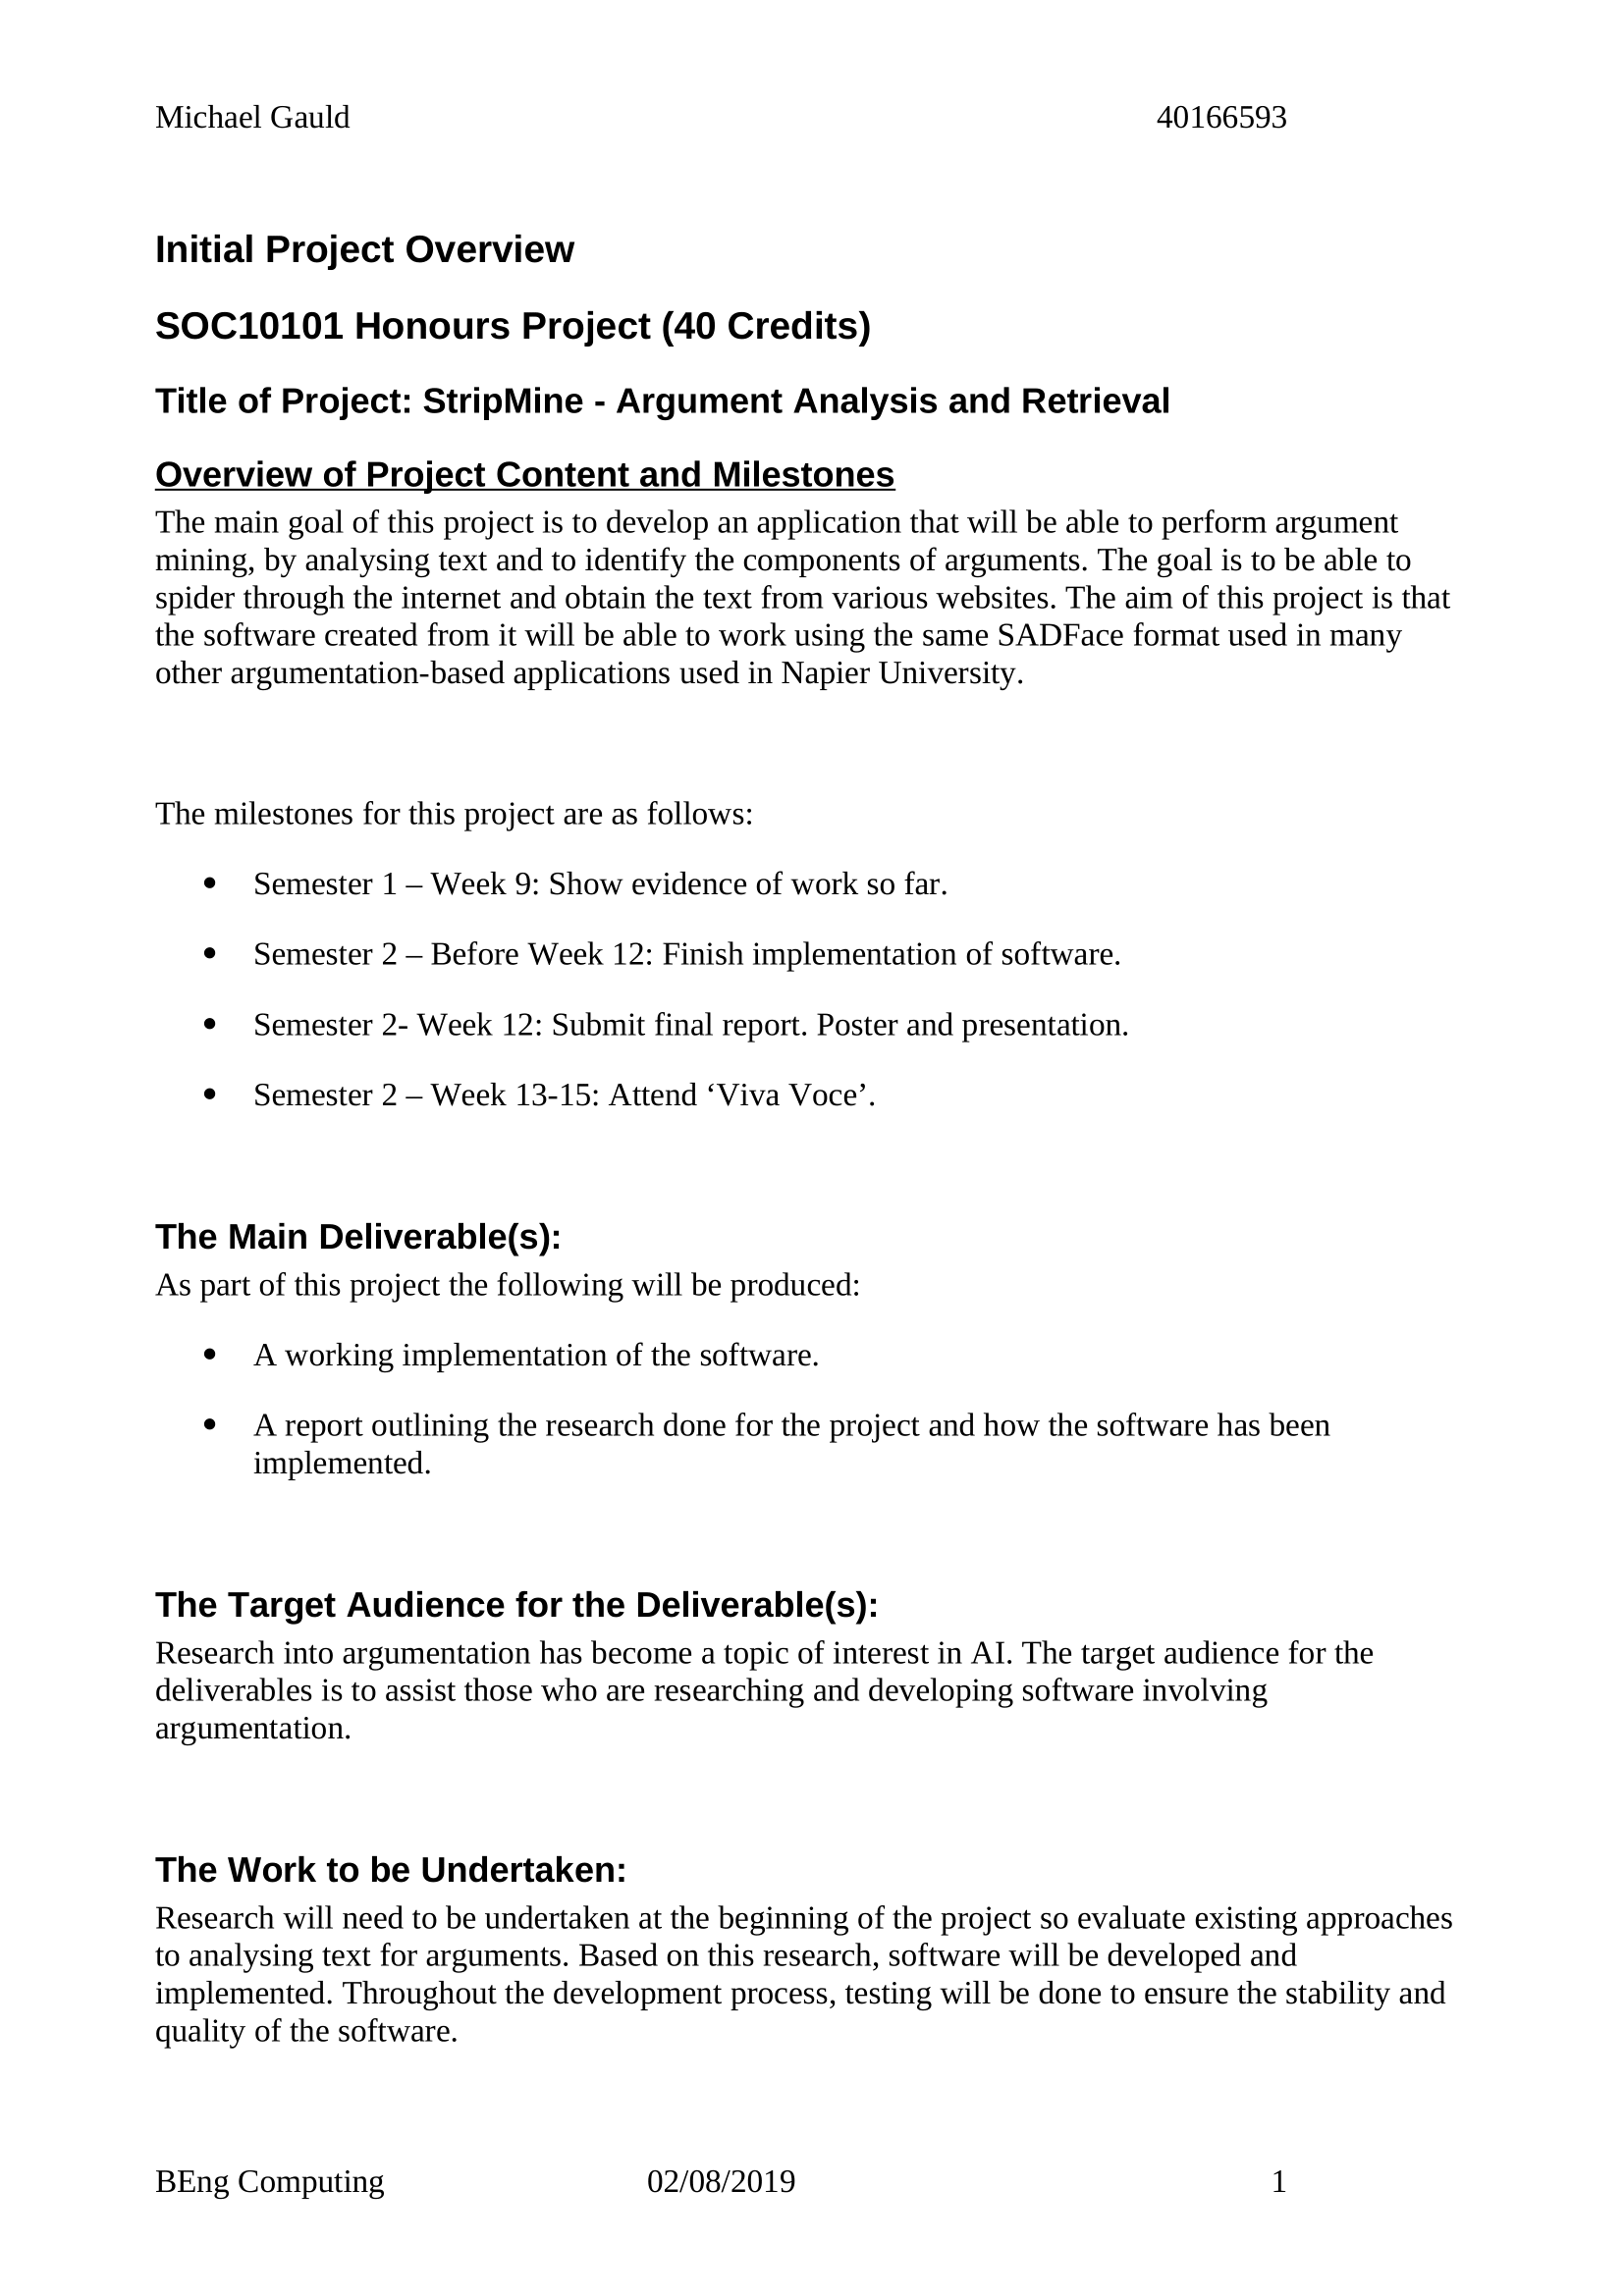
\includegraphics[scale=0.22]{Report/graphics/IPO-1.png}
\newpage
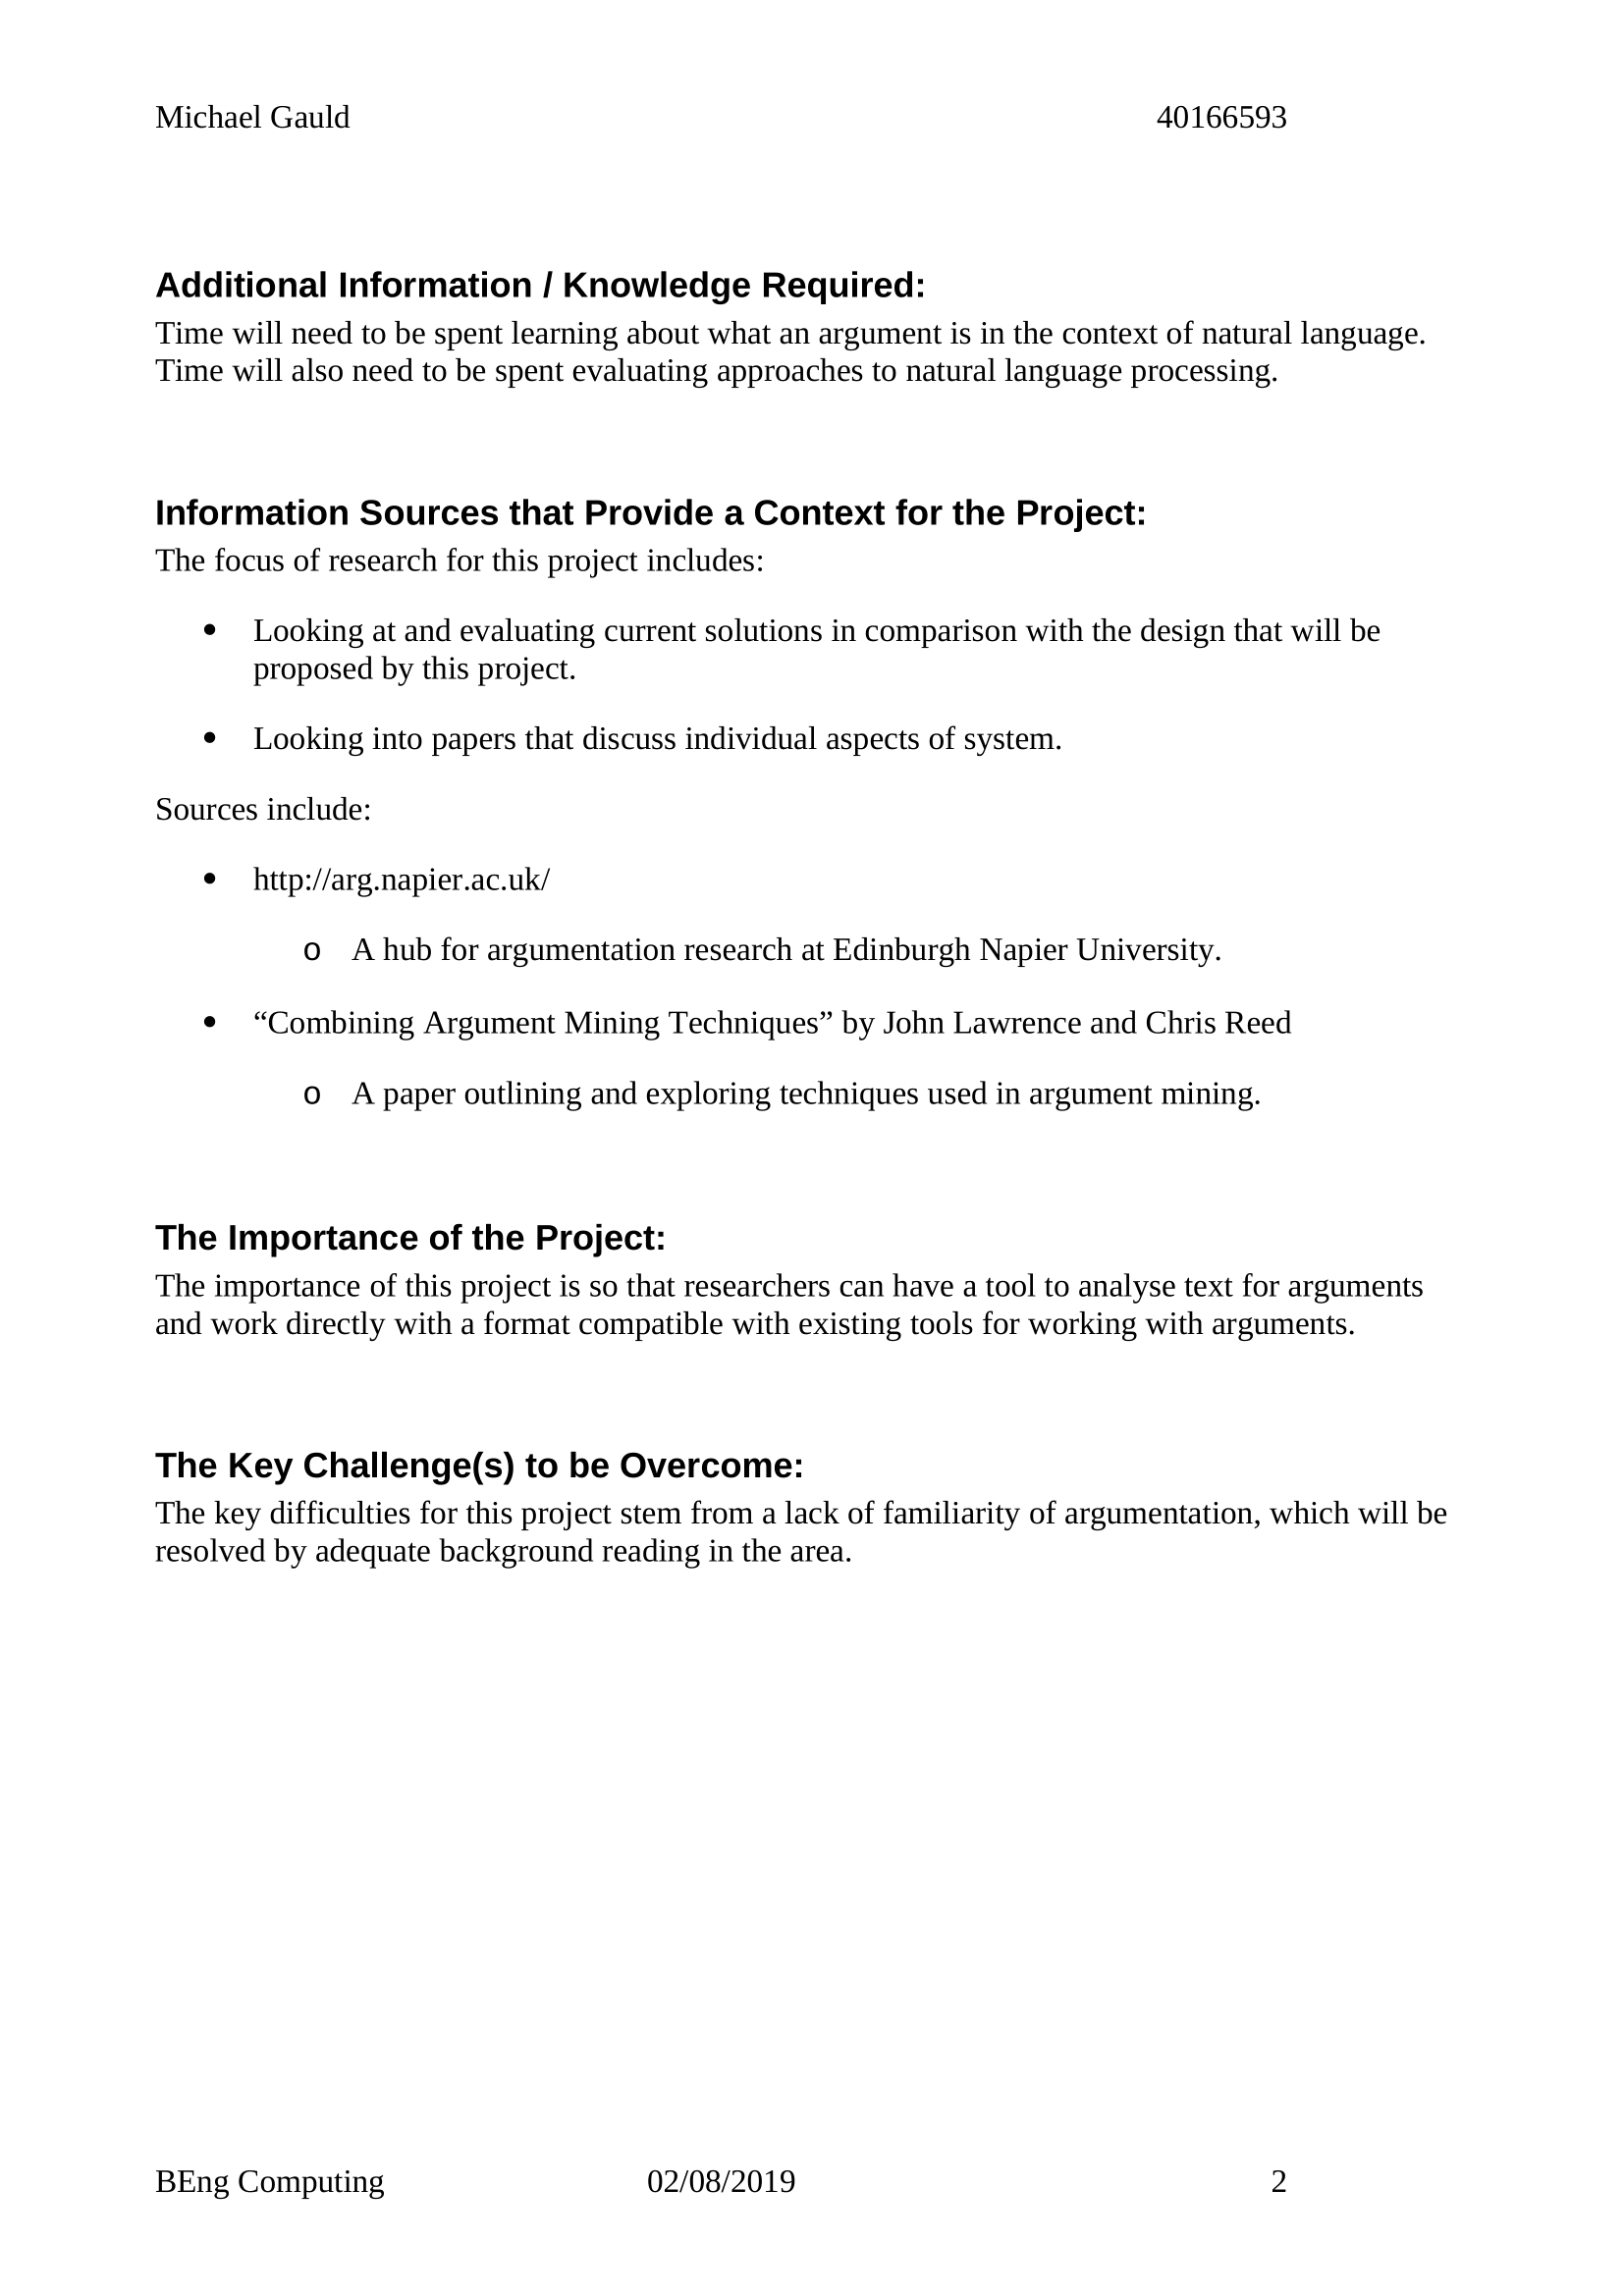
\includegraphics[scale=0.25]{Report/graphics/IPO-2.png}

\newpage
\section{Second Formal Review Output}
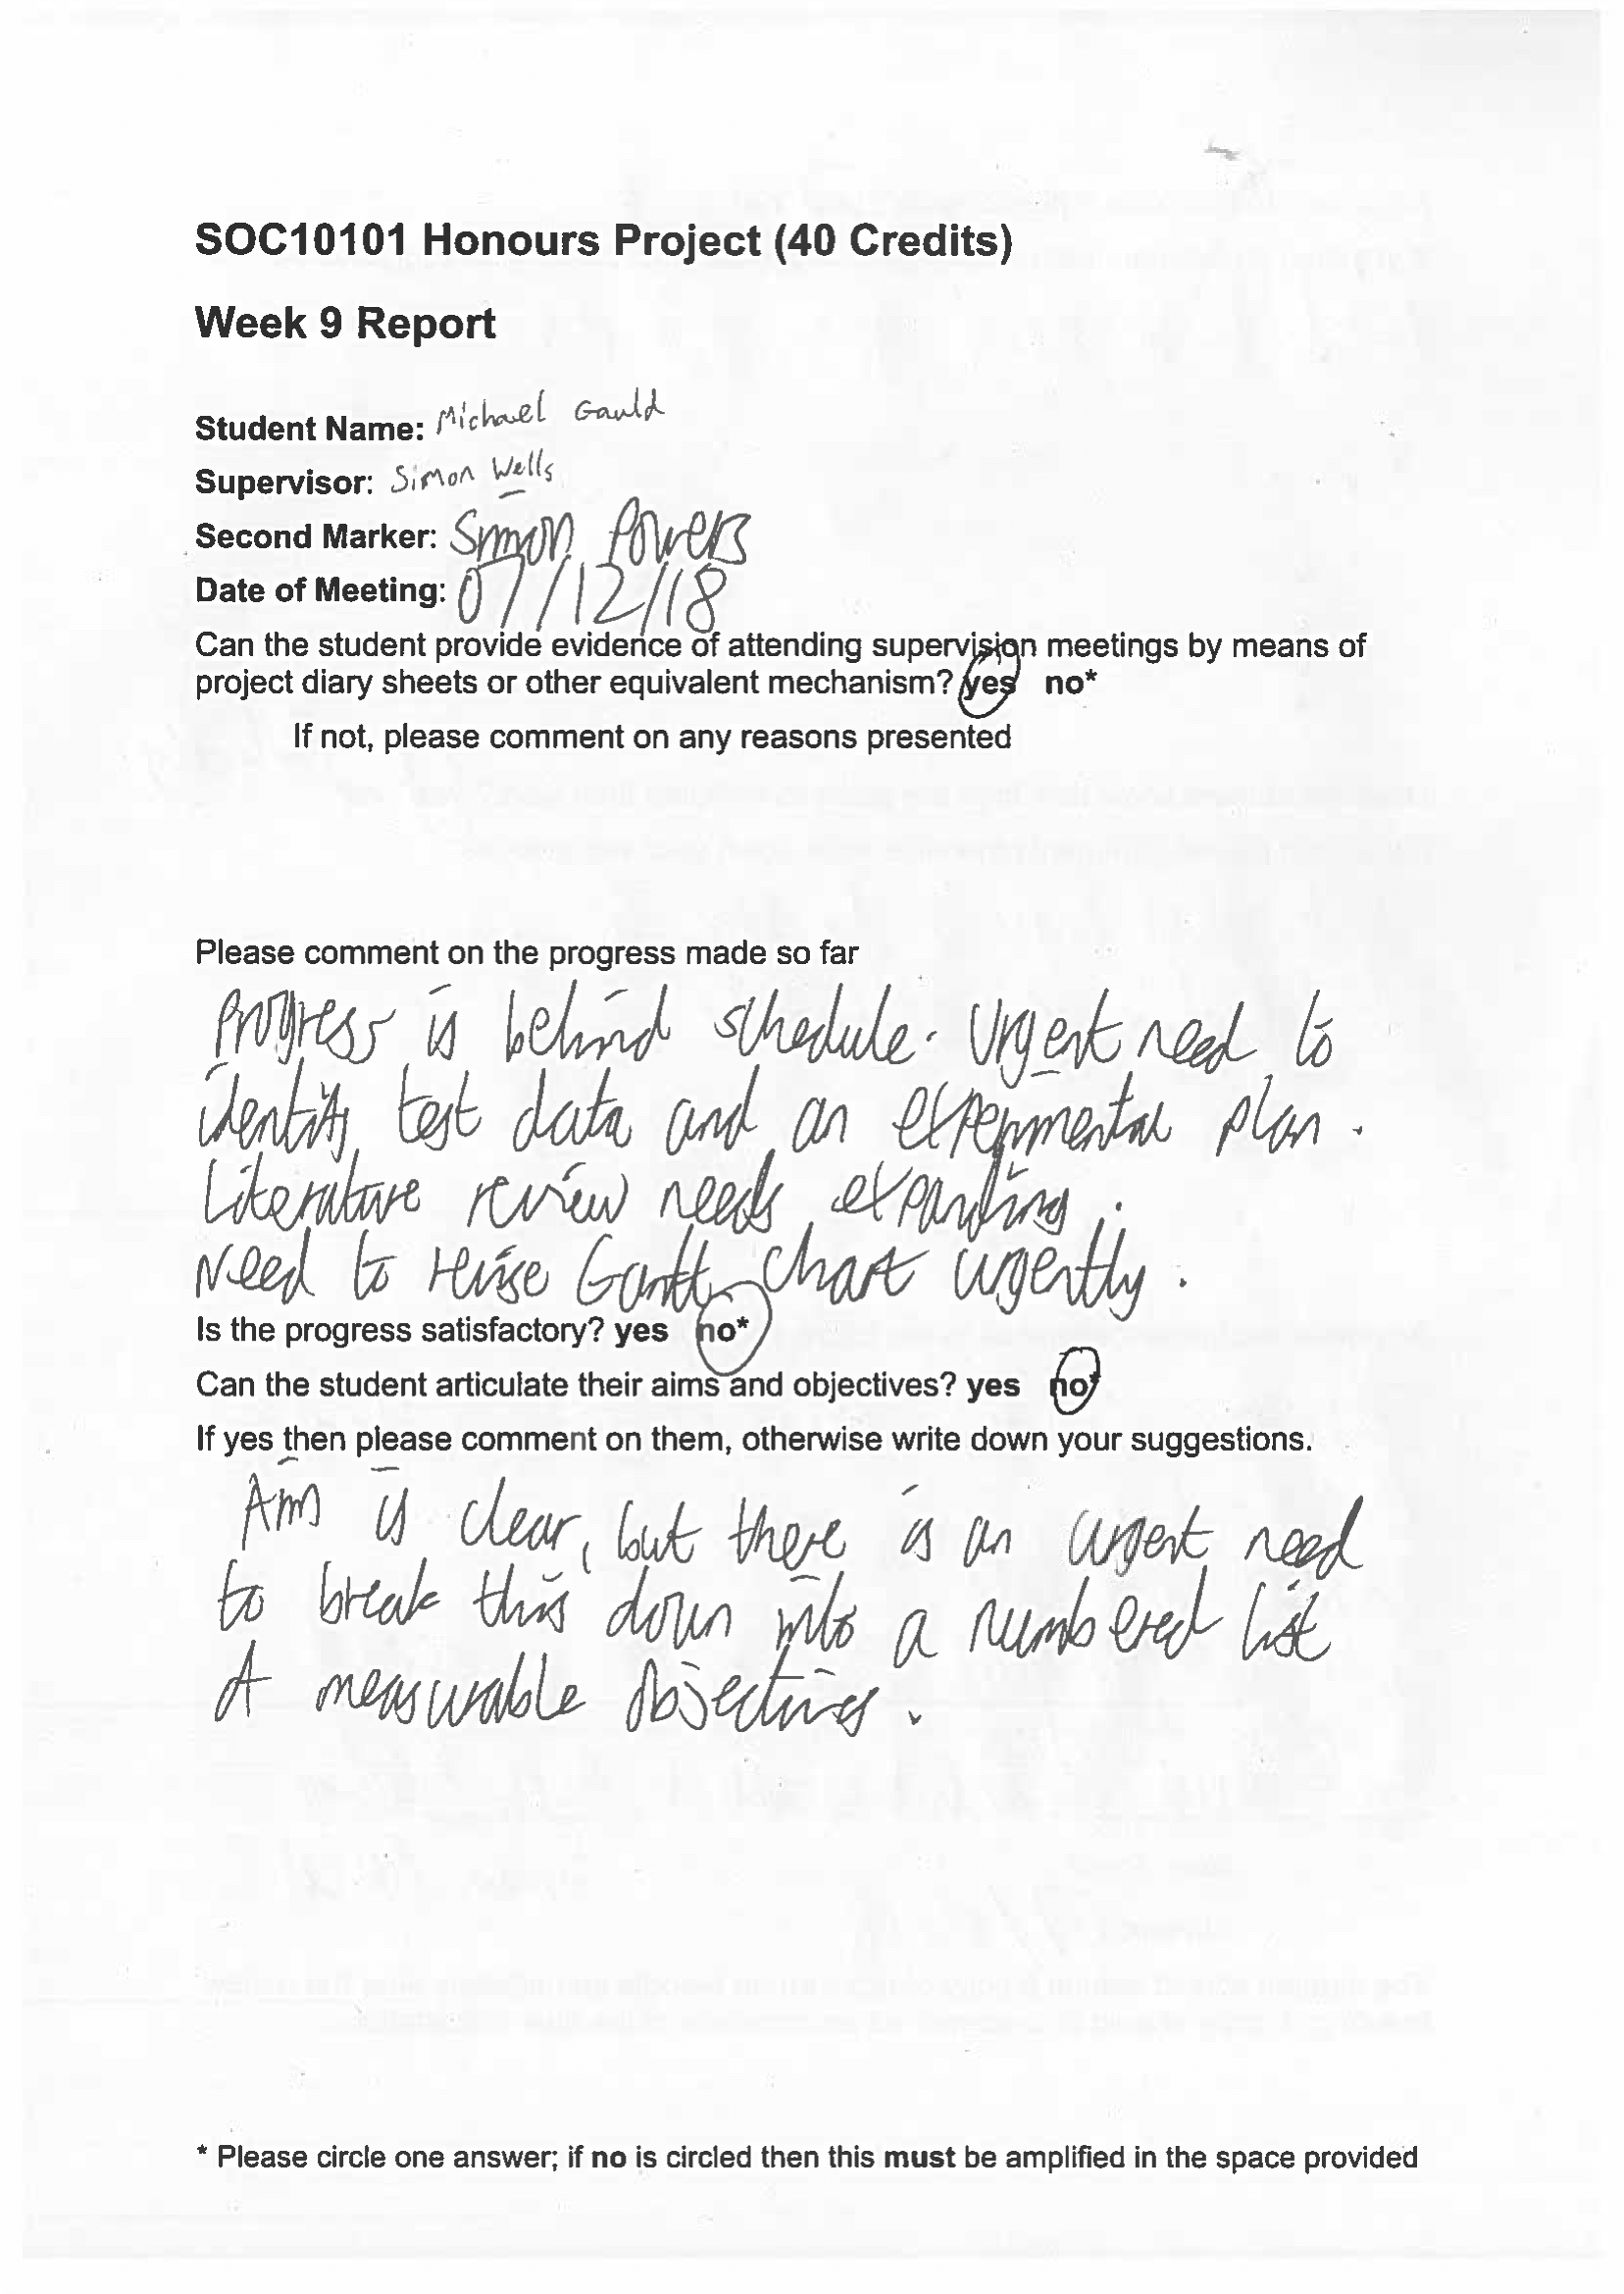
\includegraphics[scale=0.25]{Report/graphics/Review-1.png}
\newpage
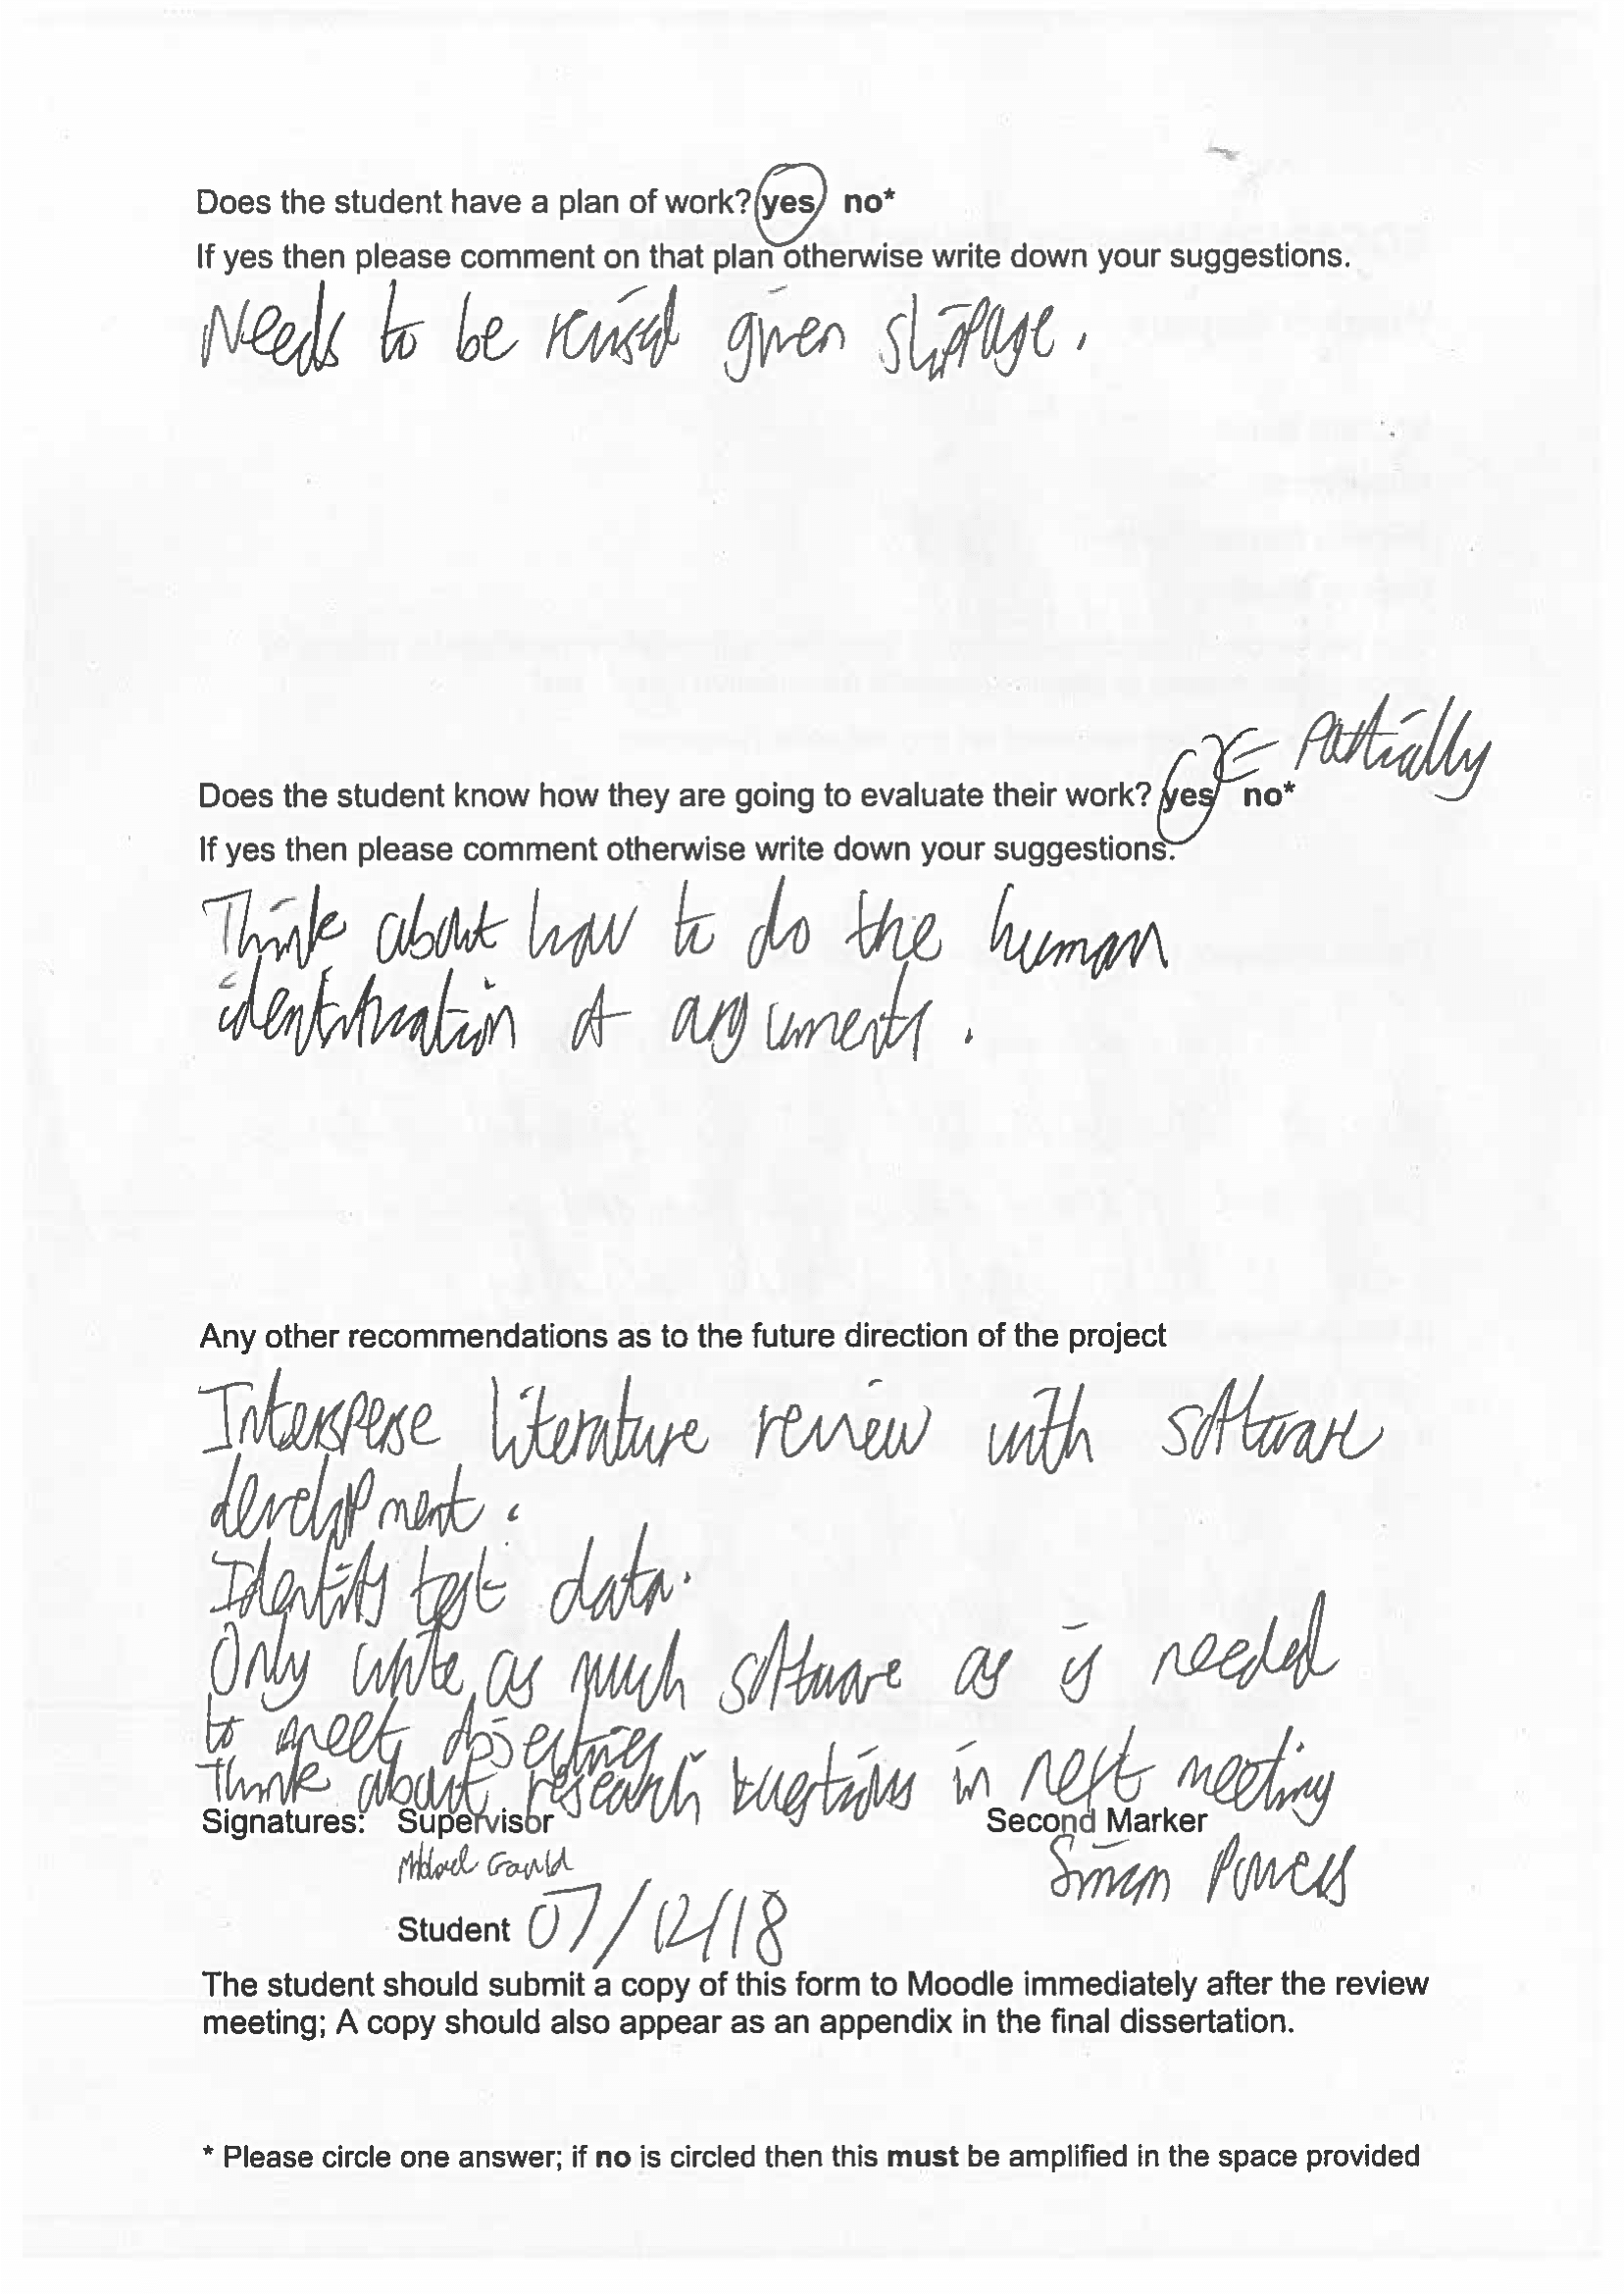
\includegraphics[scale=0.25]{Report/graphics/Review-2.png}

\newpage
\section{Diary Sheets (or other project management evidence)}
Insert diary sheets here together with any project management plan you have

\newpage
\section{Appendix 4 and following}
insert content here and for each of the other appendices, the title may be just on a page by itself, the pages of the appendices are not numbered, unless an included document such as a user manual or design document is itself pager numbered.
\end{appendices}

\end{document}
